%----------------------------------------------------------------------------------------
%	MODULE INFORMATION
%----------------------------------------------------------------------------------------

% Define the top matter
\setModuleTitle{Assessing somatic mutational signatures}
\setModuleAuthors{%
  Ann-Marie Patch, QIMRBerghofer \mailto{ann-marie.patch@qimrberghofer.edu.au} \\
  Erdahl Teber, CMRI \mailto{eteber@cmri.org.au}%
}

\setModuleContributions{%
  Martha Zakrzewski \mailto{Martha.Zakrzewski@qimrberghofer.edu.au}%
}

%----------------------------------------------------------------------------------------
%	MODULE TITLE PAGE
%----------------------------------------------------------------------------------------

\chapter{\moduleTitle}

%----------------------------------------------------------------------------------------

\newpage

%----------------------------------------------------------------------------------------
%	LEARNING OUTCOMES
%----------------------------------------------------------------------------------------

\section{Key Learning Outcomes}

After completing this practical the trainee should be able to:

\begin{itemize}
  \item Visualise mutational signatures present in a cohort using somatic single nucleotide mutation data in Variant Call Format (vcf) files.
  \item Compare analysis output with published results to identify common mutational signatures.
  \item Have gained overview knowledge of how somatic signatures can help with cohort cancer analysis.
\end{itemize}

%----------------------------------------------------------------------------------------
%	MODULE RESOURCES
%----------------------------------------------------------------------------------------

\section{Resources You'll be Using}

\subsection{Tools Used}

\begin{description}[style=multiline,labelindent=0cm,align=left,leftmargin=1cm]
  \item[R-3.2.2 statistical environment] \hfill\\
    \url{https://www.r-project.org/}
  \item[with installed R packages and their dependancies] \hfill\\
  \item[SomaticSignatures R package] \hfill\\
    \url{http://bioconductor.org/packages/release/bioc/html/SomaticSignatures.html}
  \item[BSgenome.Hsapiens.UCSC.hg19] \hfill\\
    \url{http://bioconductor.org/packages/release/data/annotation/html/BSgenome.Hsapiens.UCSC.hg19.html}    
  \item[VariantAnnotation] \hfill\\
    \url{https://bioconductor.org/packages/release/bioc/html/VariantAnnotation.html}
  \item[GenomicRanges] \hfill\\
    \url{https://bioconductor.org/packages/release/bioc/html/GenomicRanges.html}
  \item[Cairo] \hfill\\
    \url{https://cran.rstudio.com/web/packages/Cairo/index.html}
\end{description}

%------------------------------------------------

\subsection{Sources of Data}

\begin{description}[style=multiline,labelindent=0cm,align=left,leftmargin=1cm]
 \item[TCGA melanoma SNV data] \hfill\\
  \url{https://tcga-data.nci.nih.gov/tcga/}
 \item[ICGC ovarian SNV data] \hfill\\
  \url{https://dcc.icgc.org/}
\end{description}
%----------------------------------------------------------------------------------------

%------------------------------------------------

\subsection{Useful Links}

\begin{description}[style=multiline,labelindent=0cm,align=left,leftmargin=1cm]
 \item[Variant Call Format (VCF) specification] \hfill\\
  \url{http://samtools.github.io/hts-specs/VCFv4.2.pdf}
\end{description}
%----------------------------------------------------------------------------------------

\newpage

%----------------------------------------------------------------------------------------
%	INTRODUCTION
%----------------------------------------------------------------------------------------

\section{Introduction}

The most common genetic model for cancer development is the accumulation of DNA mutations over time, eventually leading to the disruption or dysregulation of enough key genes that lead cells to uncontrolled growth.
Cells in our bodies accumulate DNA mutations over time due to normal aging processes and through exposure to carcinogens.
Recently researchers found a method to take all the single nucleotide mutations identified in tumour cells (somatic SNVs) and group them together by the type of the mutation and also what the neighbouring bases are. This is commonly referred to as somatic mutational signatures.

\begin{description}[style=multiline,labelindent=0cm,align=left,leftmargin=0.5cm]
\item[Common mutational processes that are regularly identified in cancer sequencing are:] \hfill\\ 
\item[Age: the aging process. These are high in C>T transitions due to deamination of methyl-cytidine.] \hfill\\
\item[Smoking: marks exposure to inhaled carcinogens and has high numbers of C>A transversions.] \hfill\\
\item[UV: UV exposure. These are also high in C>T transitions at di-pyrimidine sites.] \hfill\\
\item[BRCA: Indicates that the homologous recombination repair pathway isn�t working properly.] \hfill\\
\item[APOBEC: Thought to be marking dysregulated APOBEC enzyme activity on single stranded DNA
produced during the repair processing of other lesions such as double stand breaks.] \hfill\\ 
\item[MMR: Mismatch repair pathway not working properly. These are high in C>T mutations too.] \hfill\\
\end{description}

In cohort cancer analysis it is common to try to generate subtypes to group your data based on a particular molecular analysis such as gene expression.
The reason for doing this is to find sets of patients that have a similar form of the disease and therefore all might benefit from a particular treatment.
We can use the somatic mutational signatures analysis to group the data from a cohort of patients and tell us which genomes are most similar based on the pattern of exposures or processes that have contributed to their genome changes.
The patients don�t have to have the same type of cancer so pan-cancer studies are using this analysis to find similarities across cancer types.


%----------------------------------------------------------------------------------------
%	Preparing the R environment
%----------------------------------------------------------------------------------------

\section{Preparing the R environment}

\begin{information}
In the Alexandrov paper the mathematical framework they developed to run the non-negative matrix factorisation (NMF) required the MATLAB software.
We are going to use a version implemented in R by Gehring, called SomaticSignatures package, that is very quick and flexible but currently only accepts point mutations not insertions or deletions (indels).
In tests on our data we have found that the Somatic Signatures package in R returns very similar results to the full implementation of Alexandrov�s framework.
\end{information}


The data files you will need are contained in the subdirectory called \texttt{somatic/somatic_signatures}:

\begin{steps}
Open the Terminal and go to the \texttt{somatic_signatures} working directory:
\begin{lstlisting}
cd ~/somatic/somatic_signatures
pwd
\end{lstlisting}

In this folder you should find 12 files that end with the extension .vcf. Use the list command to make sure you can see them.
\begin{lstlisting}
ls
\end{lstlisting}
\end{steps}

\begin{note}
These files contain data extracted from the TCGA melanoma paper and Australian ICGC ovarian paper both mentioned in the introductory slides.
They have been edited in order to allow this practical to run quickly and are not good examples of VCF files.
\end{note}

\begin{steps}
Start R and set the working directory. Just start by typing R onto the command line.
\begin{lstlisting}
R
\end{lstlisting}

Load all the package libraries needed for this analysis by running the commands.
\begin{lstlisting}
library(SomaticSignatures)
library(BSgenome.Hsapiens.UCSC.hg19)
library(ggplot2)
library(Cairo)
\end{lstlisting}

Set the drictory where any output files will be generated
\begin{lstlisting}
setwd(�~/somatic/somatic_signatures�)
\end{lstlisting}
\end{steps}


%----------------------------------------------------------------------------------------
%	Loading and preparing the SNV mutation data
%----------------------------------------------------------------------------------------

\section{Loading and preparing the SNV mutation data}

\begin{note}
The mutations used in this analysis need to be high quality somatic mutations:
�	Remember the goal is to find the key mutational processes that these tumours have been exposed to, so you need to exclude germline mutations (mutations that the person was born with that can be seen in the sequencing of matched normal samples). 
�	Sequencing errors can also occur at particular DNA sequence contexts and can also be picked up using this method. To avoid this use only high quality mutation calls.
\end{note}

\begin{steps}
Read in the mutations from the 12 vcf files
\begin{lstlisting}
files <- list.files("~/somatic/somatic_signatures", pattern="vcf$", full.names=TRUE)
\end{lstlisting}

To make sure all the files are listed run the command.
\begin{lstlisting}
files 
\end{lstlisting}

You should see a list of 12 sample files.

Next read in all the genomic positions of variants in the VCF files using the vranges class.
\begin{lstlisting}
vranges <- lapply(files, function(v) readVcfAsVRanges(v,"hg19"))
\end{lstlisting}

Join all the lists of variant positions into one big data set so that it can be
processed together and look at what is contained in the concatenated vranges data
\begin{lstlisting}
vranges.cat <- do.call(c,vranges)
vranges.cat
\end{lstlisting}
\end{steps}

\begin{information}
The first line of output of the \texttt{vranges.cat} shows us that in total we have
put over 100,000 mutations recording the chromosome positions and mutation base
changes along with what sample they were seen in.
\end{information}

\begin{note}
Note there are a lot of <NA> values in this data set because we have left out
non-essential information in order to cut down on the processing time.
\end{note}

\begin{steps}
Next we need to ensure all the positions in the vranges object have been recorded
in UCSC notation form so that they will match up with the reference we are using. 
\begin{lstlisting}
vranges.cat <- ucsc(vranges.cat)
\end{lstlisting}
\end{steps}

\begin{note}
It is always important to select the correct reference for your data.
\end{note}

\begin{steps}
We can print out how many mutations we have read in for each of the cancer samples we are using by using the command.
\begin{lstlisting}
print(table(sampleNames(vranges.cat)))
\end{lstlisting}
\end{steps}

\begin{information}
We have now added all the positional and base change information now we can
use the reference and the position of the mutation to look up the bases on
either side of the mutation i.e. the mutation context.
\end{information}

\begin{steps}
Run the mutationContext function of SomaticSignatures.
\begin{lstlisting}
mc <- mutationContext(vranges.cat, BSgenome.Hsapiens.UCSC.hg19)
\end{lstlisting}

We can inspect what information we had added to the vranges.cat
object by typing �mc� on the command line. Notice that the mutation
and its context have been added to the last two columns.
\begin{lstlisting}
mc
\end{lstlisting}

%----------------------------------------------------------------------------------------
%	understanding mutation context
%----------------------------------------------------------------------------------------
\section{SNV mutation context}

\begin{informtaion}
There are a total of 96 possible mutations and context combinations.
We can calculate this by listing out the six possible types of single
nucleotide mutations:

A->C	the reverse compliment rule means (T->G) is in this group
A->G	includes (T->C)
A->T	includes (T->A)
C->A	includes (G->T)
C->G	includes (G->C)
C->T	includes (G->C)

The neighbouring bases, on either side of a mutation, are referred to as the mutation context. 
There are 16 possible combinations of mutation contexts. Here [.] stands for one of the mutations listed above.

A[.]A		C[.]A		G[.]A		T[.]A
A[.]C		C[.]C		G[.]C		T[.]C
A[.]G		C[.]G		G[.]G		T[.]G
A[.]T		C[.]T		G[.]T		T[.]T

Now if we substitute the [.]�s with each of the 6 different mutations you will find there are 96 possible types of combined mutations and contexts (6 x 16). 

Start by substituting [.] for the A->C mutation type

	A[A->C]A	C[A->C]A
	A[A->C]C	C[A->C]C
	A[A->C]G	C[A->C]G and so on��.
	A[A->C]T

We assign all the somatic mutations identified in a single tumour to one of these categories and total up the number in each.
\end{information}

\begin{question}
What about a mutation that looks like G[T>G]A, where should this go?
Hint remember to reverse compliment all the nucleotides.
\end{question}

\begin{answer}
    In the T[A->C]C context count.
\end{answer}

\begin{steps}
Now we have all the information that is needed for each sample we can make a matrix
that contains counts of mutations in each of the 96 possible combinations of
mutations and contexts counting up the totals separately for each sample

\begin{lstlisting}
mm <- motifMatrix(mc, group = "sampleNames", normalize=TRUE)
dim(mm)
\end{lstlisting}
\end{steps}

The output of the \texttt{dim(mm)} command show us that there are 96 rows (these are the context values)
and 12 coloumns which are the 12 samples.


%----------------------------------------------------------------------------------------
%	running the NMF analysis
%----------------------------------------------------------------------------------------
\section{Running the NMF analysis}

Using the matrix we have made we can now run the non-negative matrix factorisation (NMF)
process that attempts to find the most stable, grouping solutions for all of the combinations
of mutations and contexts. It does this by trying to find similar patterns, or profiles,
amongst the samples to sort the data into firstly just 2 groups. This is repeated to get
replicate values for each attempt and then separating the data by 3 groups, and then 4 and so on.  

\begin{note}
These parameter choices have been made to keep running time short for this practical.
If you have more samples from potentially diverse sources you may
need to run with a larger range of signatures and with more replicates.
\end{note}

\begin{steps}
to find out how many signatures we have in the data run the command.
\begin{lstlisting}
gof_nmf <- assessNumberSignatures(mm, 2:10, nReplicates = 5)
\end{lstlisting}

Visualise the results from the NMF processing by making a pdf of the plot
\begin{lstlisting}
Cairo(file="plotNumberOfSignatures.pdf", type="pdf", units="in", width=9, height=8, dpi=72)
plotNumberSignatures(gof_nmf)
dev.off()
\end{lstlisting}

Open up the PDF and examine the curve.
The plotNumberOfSignatures PDF that will have been made in the working directory that you set up at the beginning
\end{steps}

\begin{figure}[H]
\centering
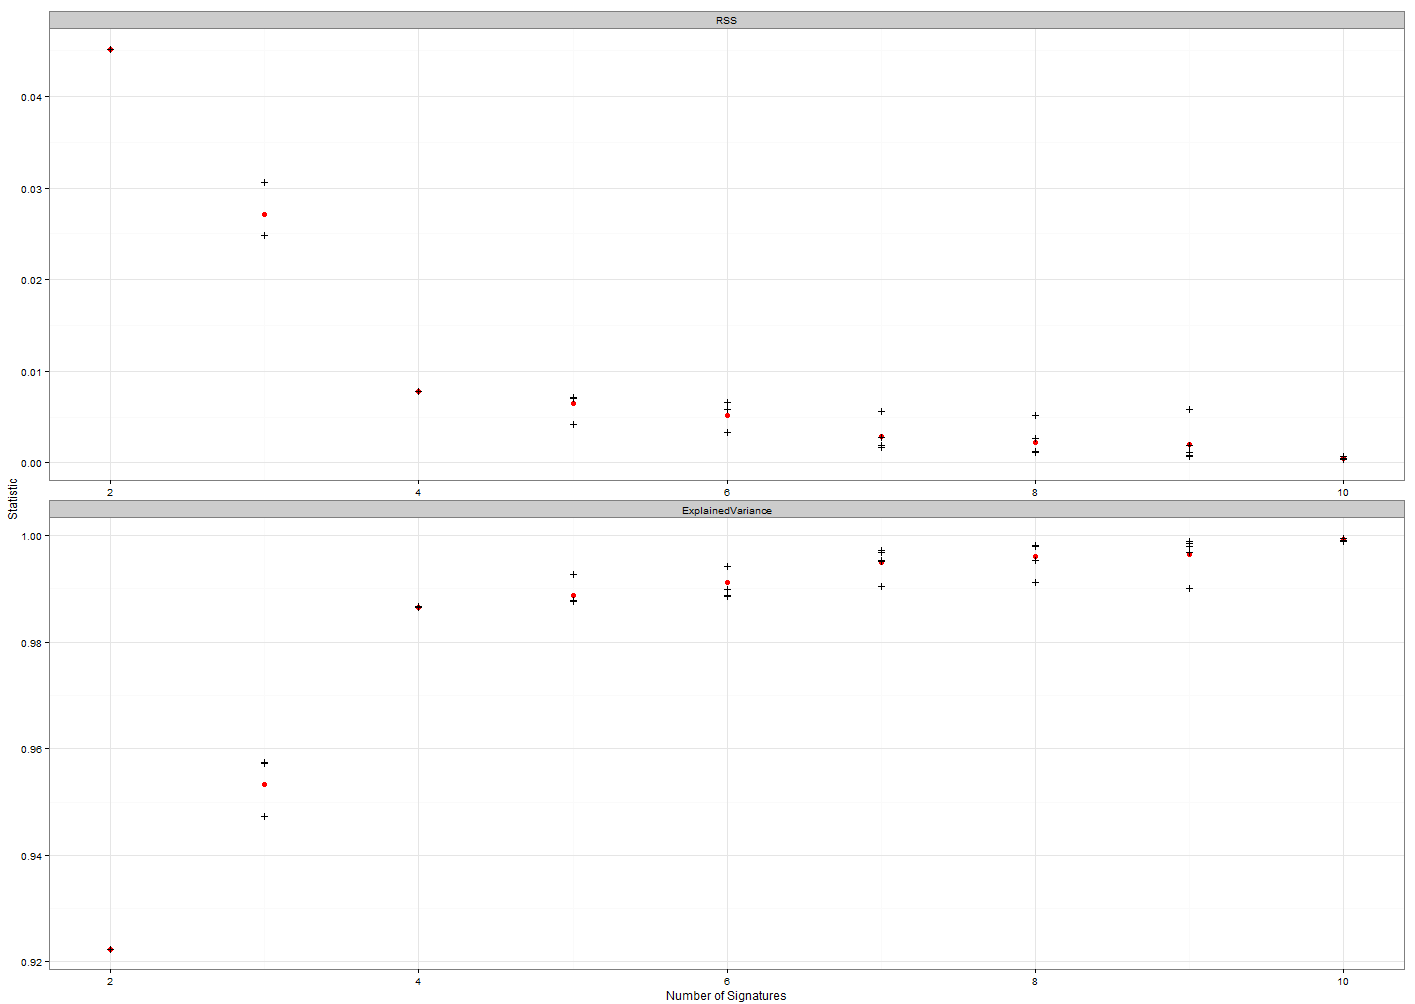
\includegraphics[width=0.8\textwidth]{handout/numberofsignatures.png}
\caption{This plot is used to find the number of signatures that is likely
to be the best grouping solution. The top plot shows the decreasing residual
sum of squares for each increasing number of signatures and the bottom plot the
increasing explained variance as the number of potential signatures increases.
Ideally the best solution will be the lowest number of signatures with
a low RSS and a high explained variance.}
\label{Figure 1:Number of signatures plot}
\end{figure}

Look at the y-axis scale on the bottom panel of Figure 1.
The explained variance is already very high and so close to finding
the correct solution for the number of signatures even with just 2.
The error bars around each point are fairly small considering we have
a very small sample set. Deciding how many signatures are present can
be tricky but here let�s go for 3.
This is where the gradient of both curves have started to flatten out.

\begin{steps}
Now run the NMF again but this time stipulating that you want to group the data into 3 different mutational signatures.
\begin{lstlisting}
sigs_nmf = identifySignatures(mm, 3, nmfDecomposition)
\end{lstlisting}

Visualise the shape of the profiles for these 3 signatures
\begin{lstlisting}
Cairo(file="plot3Signatures.pdf", type="pdf", units="in", width=10, height=8, dpi=72)
plotSignatures(sigs_nmf,normalize=TRUE, percent=FALSE) + ggtitle("Somatic Signatures: NMF - Barchart") + scale_fill_brewer(palette = "Set2")
dev.off()
\end{lstlisting}

open up the plot3Signatures pdf that will have been made in the working directory.
\end{steps}

\begin {information}
You should have generated a plot with three signature profiles obtained from the NMF processing
of the test dataset.

The 96 possible mutation/context combinations are plotted along the x
axis arranged in blocks of 6 lots of 16 (see information above).
The height of the bars indicates the frequency of those particular
mutation and context combinations in each signature.

Although the section colours are different to the plot you have generated the
mutations are still in the same order across the plot. 
\end{information}

%----------------------------------------------------------------------------------------
%	Results interpretation
%----------------------------------------------------------------------------------------
\section{Interpreting the signature results}

In their paper Alexandrov et al used this analysis to generate profiles from the data for
more than 7000 tumour samples sequenced through both exome and whole genome approaches.
They were able to group the data to reveal which genomes have been exposed to similar
mutational processes contributing to the genome mutations.

\begin{figure}[H]
\centering
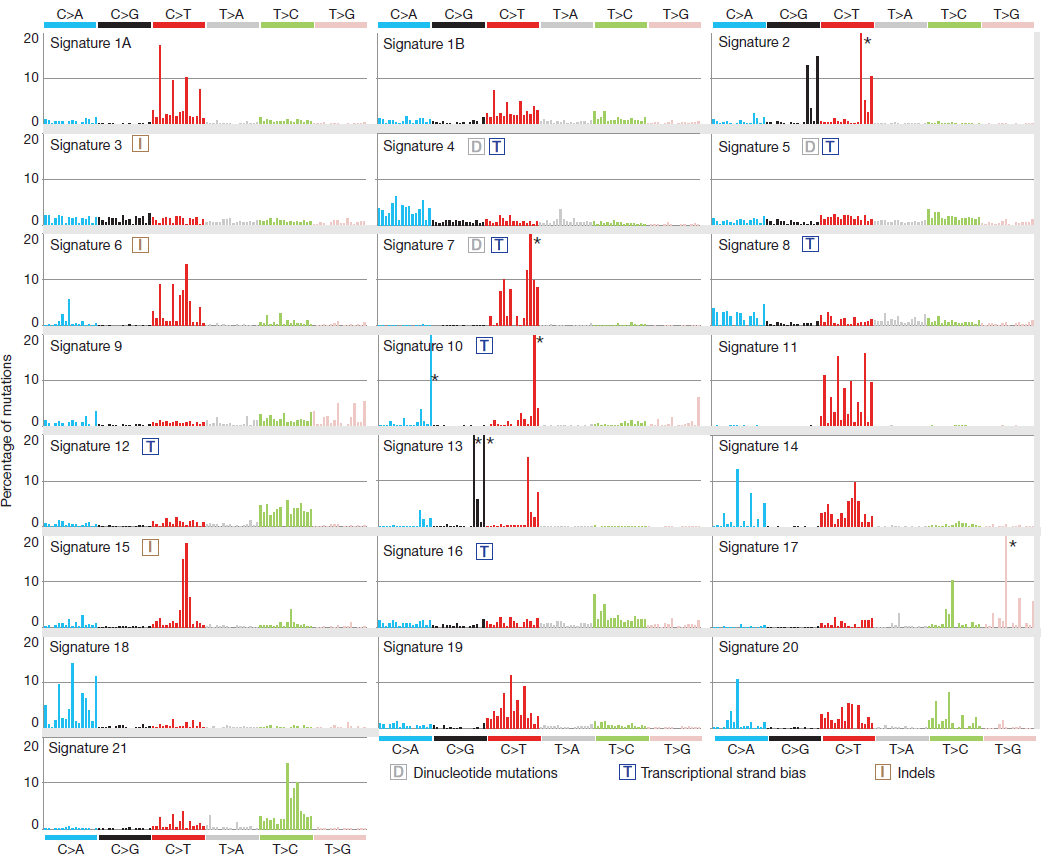
\includegraphics[width=0.8\textwidth]{handout/alexandrov_nature.png}
\caption{The 96 possible mutation/context combinations are plotted along the x axis
arranged in blocks of 6 lots of 16. The height of the bars indicates the frequency
of those particular mutation and context combinations in each signature}
\label{Figure 2. 21 signature patterns identified from the analysis of more
than 7000 different tumours from Alexandrov et al. Nature 2013.}
\end{figure}

\begin{question}
Can you match up, by eye, the profile shapes against a selection of known
mutational signatures supplied (figure 2)?

Try to match up the patterns made by the positions of the highest peaks for each signature.
\end{question}

\begin{answer}
Alexandrov signature 7 matches with our signature 1

Alexandrov signature 13 matches with our signature 2

Alexandrov signature 3 matches with our signature 3
\end{answer}

Now use the table from Alexandrov et al to identify wich mutational
processes our three generated signatures have been asscoaiated with.

\begin{figure}[H]
\centering
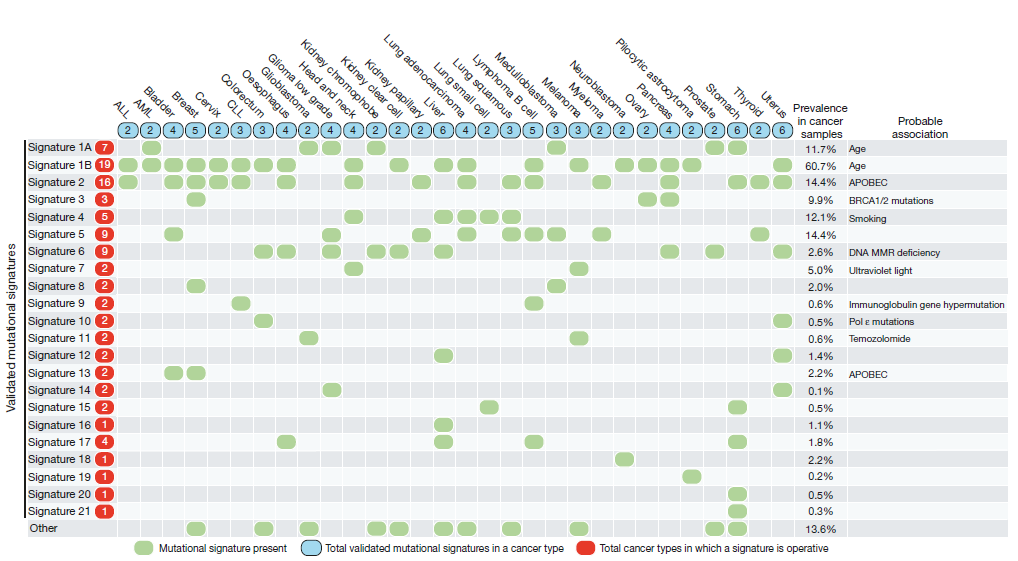
\includegraphics[width=0.8\textwidth]{handout/mutational_processes.png}
\caption{The 21 signatures identified are indicated as rows with the number corresponding
to Figure2 on the left. The types of tumours used in the analysis are listed as coloumns.
A green dot at the intersection of a signature and tumour indicates the signature was
identified in that sample type. Where verified the mutational process is listed on the right.}
\label{Figure 3 Table indicating the probable association of the identified signatures
with mutational processes and the origin site of the cancer samples
from Alexandrov et al. Nature 2013.}
\end{figure}

\begin{question}
What mutational mechanisms have been associated with the signatures that you have generated?
\end{question}

\begin{answer}
Our signature 1 (AS7) is associated with Ultraviolet radiation damage to DNA. This has previously been identified in Head and Neck and Melanoma cancer samples.

Our signature 2 (AS 13) is associated with the activity of anti-viral APOBEC enzymes. This has previously been seen in Breast and Bladder cancer samples.

Our signature 3 (AS3) is associated with BRCA1 and BRCA2 mutations, i.e. the homologous recombination repair pathway not working properly. This has been seen in Breast, Ovarian and Pancreas cancer samples.
\end{answer}

begin{steps}
Now we can plot out the results for the individual samples in our dataset to show what proportion of their mutations have been assigned to each of the signatures.
\begin{lstlisting}
Cairo(file="PlotSampleContribution3Signatures.pdf", type="pdf", units="in", width=9, height=6, dpi=72)
plotSamples(sigs_nmf, normalize=TRUE) + scale_y_continuous(breaks=seq(0, 1, 0.2), expand = c(0,0))+ theme(axis.text.x = element_text(size=6))
dev.off()
\end{lstlisting}

If you don't have time to carry out the advanced questions you can
exit R and return to the normal terminal command line.
\begin{lstlisting}
quit()
n
\end{lstlisting}


Open the resulting plot. This shows the results for the mutation grouping for each sample.
The samples are listed on the x-axis and the propotion of all mutations for that
sample is shown on the y-axis. The colours of the bars indicate what proportion of the
mutations for that sample were grouped into each of the signatures. The colour
that makes up most of the bar for each sample is called its �major signature�.
\end{steps}

\begin{information}
The data you have been using contains samples from High Grade Serous Ovarian Carcinomas and Cutaneous Melanoma. 
\end{information}

\begin{question}
Using the major signature found for each sample can you guess which are ovarian and which are melanoma samples?
\end{question}

\begin{answer}
Samples 9-12 have the majority signature of our signature 1. This is the UV signature and so these are likely to be Melanoma samples.

Samples 4-8 have the majority signature of our signature 3. This is the BRCA signature and these are most likely to be ovarian samples.

Samples 1-3 have the majority signature of our signature 2. This is the APOBEC signature indicating activity of the anti-viral APOBEC enzymes. These are less likely to be from cutaneous melanoma because they have very few UV associated mutations although it could possibly be from a different subtype. However it is much more likely that these will be ovarian tumours as this APOBEC signature has been seen in breast tumours which can be similar to ovarian cancers in terms of the mutated genes.
\end{answer}


begin{question}
This is an open question of discussion at the end of the practical.

How can this analysis be useful for cancer genomics studies?
end{question}

\begin{advanced}
Now rerun the process this time using 4 signatures as the solution.
\begin{information}
Hint: you don�t have to start back at the beginning but you can jump
to the step where you run the NMF but this time for 4 instead of 3
signatures. Then continue through making the plots.

You will need to change the name of each plot you remake with 4
signatures because Cairo won't let you overwrite and exsiting file.
\end{information}
\begin{question}
Can you find a good match in the set of known signatures for all 4 patterns? 

Can you find a verified process for all of the profiles you are seeing? 
\end{question}
\end{advanced}

%----------------------------------------------------------------------------------------
%	REFERENCES
%----------------------------------------------------------------------------------------

\section{References}

\begin{description}[style=multiline,labelindent=0cm,align=left,leftmargin=1cm]
 \item[Alexandrov et al. Nature 2013] \hfill\\
  \url{http://www.nature.com/nature/journal/v500/n7463/pdf/nature12477.pdf}
 \item[Gehring et al. Bioinformatics 2015] \hfill\\
  \url{http://bioinformatics.oxfordjournals.org/content/early/2015/07/31/bioinformatics.btv408.full}
\end{description}
